% This must be in the first 5 lines to tell arXiv to use pdfLaTeX, which is strongly recommended.
% \pdfoutput=1
% In particular, the hyperref package requires pdfLaTeX in order to break URLs across lines.

\documentclass[11pt]{article}

% Remove the "review" option to generate the final version.
\usepackage[final]{ACL2023}

% Standard package includes
\usepackage{times}
\usepackage{latexsym}

% For proper rendering and hyphenation of words containing Latin characters (including in bib files)
\usepackage[T1]{fontenc}
% For Vietnamese characters
% \usepackage[T5]{fontenc}
% See https://www.latex-project.org/help/documentation/encguide.pdf for other character sets

% This assumes your files are encoded as UTF8
\usepackage[utf8]{inputenc}
% \usepackage[round]{natbib}

% This is not strictly necessary, and may be commented out.
% However, it will improve the layout of the manuscript,
% and will typically save some space.
\usepackage{microtype}

% This is also not strictly necessary, and may be commented out.
% However, it will improve the aesthetics of text in
% the typewriter font.
\usepackage{inconsolata}

% For including images and graphics
\usepackage{graphicx}

\hypersetup{
    citecolor=blue 
}
% If the title and author information does not fit in the area allocated, uncomment the following
%
%\setlength\titlebox{<dim>}
%
% and set <dim> to something 5cm or larger.

\title{A Survey on Enhancement and Efficiency in Retrieval-Augmented Generation}

% Author information can be set in various styles:
% For several authors from the same institution:
% \author{Author 1 \and ... \and Author n \\
%         Address line \\ ... \\ Address line}
% if the names do not fit well on one line use
%         Author 1 \\ {\bf Author 2} \\ ... \\ {\bf Author n} \\
% For authors from different institutions:
% \author{Author 1 \\ Address line \\  ... \\ Address line
%         \And  ... \And
%         Author n \\ Address line \\ ... \\ Address line}
% To start a seperate ``row'' of authors use \AND, as in
% \author{Author 1 \\ Address line \\  ... \\ Address line
%         \AND
%         Author 2 \\ Address line \\ ... \\ Address line \And
%         Author 3 \\ Address line \\ ... \\ Address line}

\author{
  Guiyan He \\
  Texas A\&M University \\
  UIN: 136005919 \\
  \texttt{guiyanhe@tamu.edu}
  \And
  Yi-Hsin Chiang \\
  Texas A\&M University \\
  UIN: 137001082 \\
  \texttt{yihsin.chiang@tamu.edu}
  \And
  Xiaochuan (Sean) Ge \\
  Texas A\&M University \\
  UIN: 937006752 \\
  \texttt{xiaochuan@tamu.edu}}


\begin{document}
\maketitle
\pagestyle{plain}
\begin{abstract}
Retrieval-Augmented Generation (RAG) has emerged as a critical approach for enhancing large language models with external knowledge. While RAG systems are widely adopted, they face significant challenges in reliability, accuracy, and computational efficiency. This survey systematically examines recent advances in RAG optimization through two primary dimensions: Enhancement (quality and robustness) and Efficiency (speed and resource usage). We provide detailed analysis of representative methods including Self-RAG, RE-RAG, CRAG, FLARE, GraphRAG, RAFT, LLMLingua, and Speculative RAG, offering practical insights for both researchers exploring open problems and engineers implementing production systems. Our focused approach addresses gaps in existing literature by emphasizing concrete optimization techniques rather than broad architectural overviews, revealing emerging trends from static retrieval systems toward agentic, self-correcting architectures.
\end{abstract}

\section{Introduction}

Retrieval-Augmented Generation (RAG) represents a paradigm shift in how large language models (LLMs) interact with external knowledge. By combining the generative capabilities of LLMs with the precision of information retrieval systems, RAG addresses fundamental limitations of standalone language models, including knowledge staleness, hallucination, and limited domain expertise. The basic RAG architecture operates through a simple yet powerful mechanism: given a user query, a retriever fetches relevant documents from an external knowledge base, which are then concatenated with the original query to augment the prompt for a generative model. This approach enables LLMs to ground their responses in verifiable, up-to-date information without requiring expensive retraining.

Despite widespread adoption across industries—from customer support chatbots to medical question-answering systems—RAG faces critical bottlenecks that hinder practical deployment. Reliability remains a primary concern when retrieved documents contain noise, contradictory information, or irrelevant content, leading to degraded output quality or even amplified hallucinations. Additionally, computational costs associated with processing lengthy contexts, performing multiple retrieval operations, and running large generative models create significant efficiency challenges, particularly for latency-sensitive applications and resource-constrained deployments.

\subsection{Motivation and Scope}

The motivation for this survey stems from a fundamental observation: success in RAG deployment depends critically on optimization. As one industry practitioner noted, "Success depends on optimization." While RAG offers compelling theoretical advantages, real-world applications demand systems that achieve both high accuracy and computational efficiency—goals that often exist in tension with one another.

Current literature provides valuable broad surveys of RAG architectures and applications. However, practitioners implementing production systems often find these surveys lack sufficient depth on specific optimization techniques. When should one employ query rewriting versus document reranking? How can prompt compression maintain semantic coherence while achieving 20x reduction? What are the trade-offs between drafter-verifier architectures and single-model approaches? These practical questions often go unanswered in existing surveys.

This survey addresses these gaps by analyzing RAG through two specific, actionable dimensions:

\textbf{Enhancement} focuses on improving quality and robustness through two complementary approaches. First, retriever optimization encompasses techniques for improving the relevance and utility of retrieved information, including advanced query rewriting methods, hybrid search models combining dense and sparse retrieval, context-aware retrieval strategies, and web search fallback mechanisms. Second, generator optimization covers methods for helping language models better synthesize retrieved context, focusing on improving factual accuracy, handling noisy or contradictory sources, integrating self-reflection mechanisms, and filtering irrelevant information before generation.

\textbf{Efficiency} addresses speed and resource consumption through data-centric and model-centric approaches. Data-centric optimizations organize, structure, or compress input before it reaches the model, including sophisticated prompt compression techniques, efficient indexing strategies, and caching mechanisms. Model-centric approaches modify the inference pipeline or architecture itself, employing techniques such as speculative decoding with drafter-verifier architectures, parallel processing strategies, and dynamic retrieval triggering based on confidence thresholds.

Our target audience spans two critical communities. For researchers, we identify open problems and emerging directions, including the need for standardized efficiency benchmarks, optimal model size combinations in compound architectures, and methods for handling contradictory information. For engineers building production systems, we provide concrete guidance on technique selection, implementation trade-offs, and performance characteristics based on real-world deployments.

\subsection{Gap in Current Literature}

Recent comprehensive surveys have made valuable contributions to understanding the RAG landscape. "Retrieval And Structuring Augmented Generation with Large Language Models" by Jiang et al. (2025) provides an extensive overview of RAG architectures and structuring techniques. "Retrieval Augmented Generation Evaluation in the Era of Large Language Models" by Gan et al. (2025) focuses on evaluation methodologies and benchmarks across different RAG configurations. These works establish important foundational understanding and taxonomies.

However, these surveys tend toward breadth over depth, covering many techniques at a high level without detailed implementation guidance. They often lack concrete examples of how to implement specific optimizations such as dynamic retrieval strategies that trigger based on model confidence, budget-aware compression that allocates different compression ratios to prompt components, or multi-agent architectures that decompose complex queries into subtasks. Additionally, most surveys organize content by component (retriever, generator, etc.) rather than by optimization goal (accuracy vs. efficiency), making it challenging to understand trade-offs.

Our survey addresses this gap through three key contributions. First, we focus strictly on optimization techniques rather than general architecture, providing actionable guidance for practitioners. Second, we organize content by optimization objective (enhancement vs. efficiency), making trade-offs explicit and enabling informed decision-making. Third, we include detailed case studies of representative techniques, explaining not just what they do but how they achieve their results and when to apply them.

\begin{figure*}[t]
  \centering
  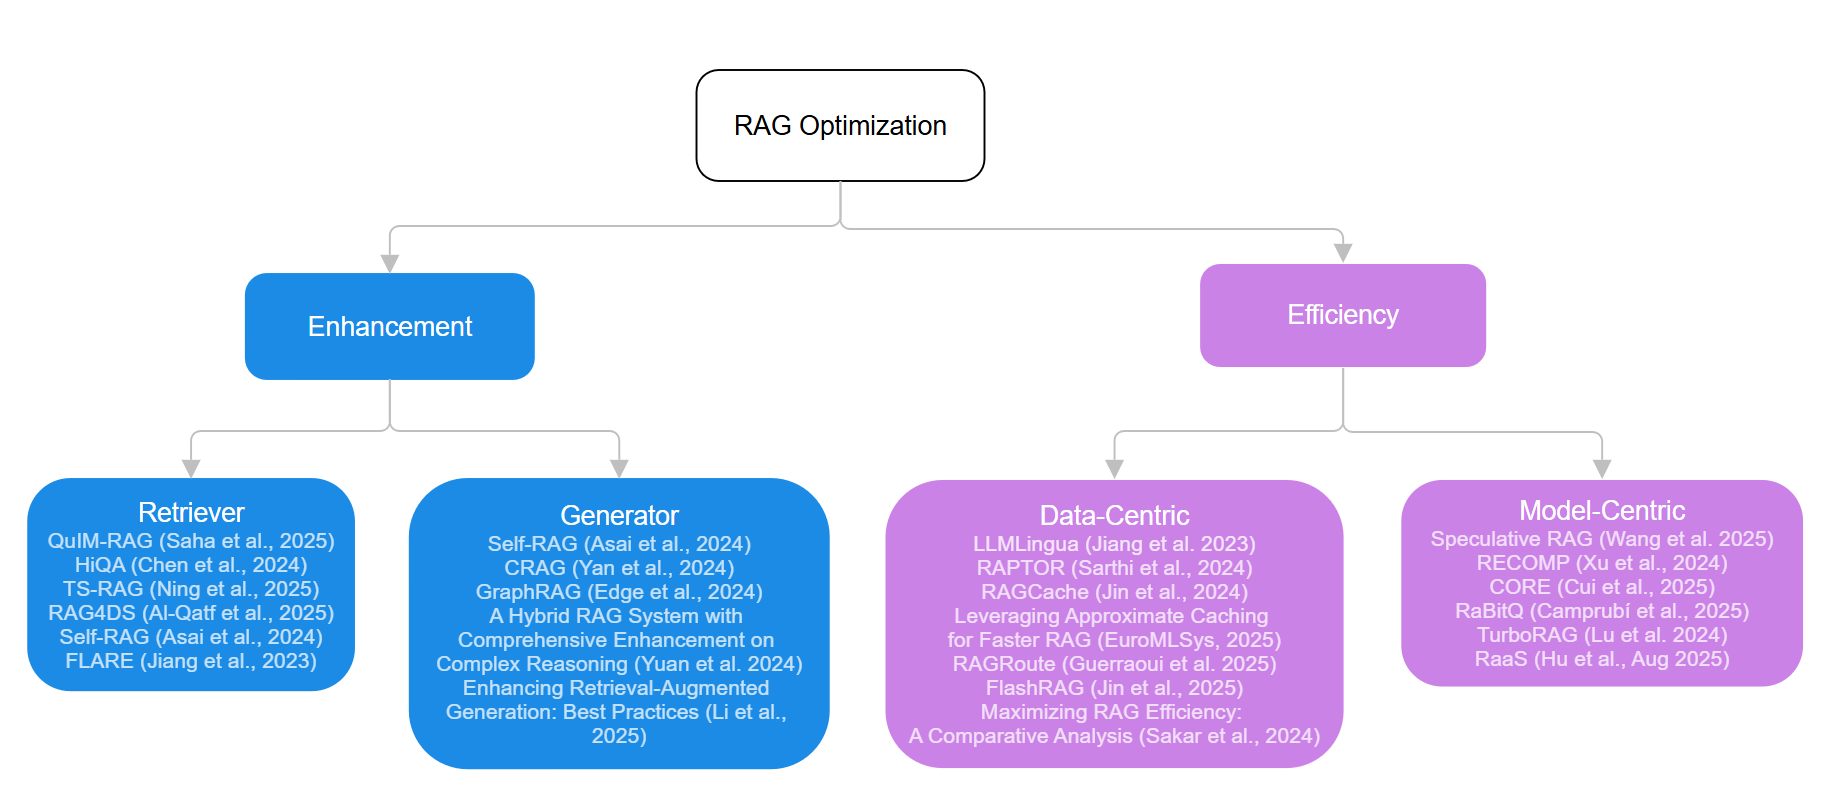
\includegraphics[width=\textwidth]{Flowchart}
  \caption{Overview of Enhancement and Efficiency Methods in RAG}
  \label{fig:fig1}
\end{figure*}

\section{Preliminaries and Foundations}

Before examining specific optimization techniques, we establish foundational understanding of the RAG framework, its core components, and evaluation methodologies.

\subsection{RAG Architecture Overview}

A typical RAG system consists of two primary components working in concert to combine retrieval precision with generation flexibility.

The \textbf{Retriever} component is responsible for fetching relevant documents or passages from a large corpus based on the input query. Modern retrievers fall into several categories based on their matching mechanisms. Dense retrieval models such as Dense Passage Retrieval (DPR) and ColBERT use learned neural embeddings to represent both queries and documents in a shared semantic space, enabling similarity-based matching that captures semantic relatedness beyond keyword overlap. Sparse retrieval models such as BM25 rely on traditional information retrieval techniques using term-based matching, offering computational efficiency and interpretability. Hybrid approaches that combine both paradigms have shown promising results by leveraging complementary strengths: sparse methods excel at exact keyword matching while dense methods capture semantic similarity.

The \textbf{Generator} is typically a large language model that takes retrieved documents as additional context and produces coherent, contextually relevant responses. Popular generator architectures include GPT variants (GPT-3, GPT-4), T5 (Text-to-Text Transfer Transformer), and BART (Bidirectional and Auto-Regressive Transformers). The generator must effectively synthesize information from multiple sources while maintaining factual accuracy, coherence, and faithfulness to the retrieved evidence. This synthesis challenge becomes particularly acute when retrieved documents contain contradictory information or when only portions of retrieved documents are relevant to the query.

\subsection{Standard RAG Pipeline}

The conventional RAG pipeline operates through a sequential process. Given a user query $q$, the retriever searches a document corpus $\mathcal{D}$ and returns the top-$k$ most relevant passages $\{d_1, d_2, ..., d_k\}$ based on a relevance scoring function. These passages are then concatenated with the original query to form an augmented prompt: $p = [q; d_1; d_2; ...; d_k]$. This augmented prompt is processed by the generator LLM to produce the final response $r$.

This simple architecture, while effective for many applications, suffers from several inherent limitations that motivate the optimization techniques surveyed in this paper. First, the retriever operates independently of the generator, potentially fetching documents that are semantically similar to the query but not actually useful for generation. Second, all retrieved documents are treated equally regardless of their actual utility, leading to context window bloat and increased inference costs. Third, the system retrieves once upfront rather than dynamically adjusting retrieval based on generation needs. Fourth, there is no mechanism for the system to critique or verify its own outputs, leading to propagation of errors when retrieval is poor.

\subsection{Datasets and Evaluation Metrics}

Common datasets used for RAG evaluation span different domains and task types. Natural Questions provides open-domain question answering pairs derived from Google search queries with answers from Wikipedia, testing systems' ability to locate and synthesize information from large document collections. TriviaQA focuses on trivia questions requiring factual knowledge, with evidence passages from Wikipedia and web documents. HotpotQA requires multi-hop reasoning where answering questions necessitates combining information from multiple documents. PubMedQA tests biomedical question answering using research paper abstracts, evaluating domain-specific performance. WebGPT provides web-based question answering with human-written answers and citations, enabling evaluation of both answer quality and attribution.

Standard evaluation metrics assess different aspects of RAG performance. Exact Match (EM) measures the percentage of generated answers that match gold standard answers exactly, providing a strict accuracy measure. F1 Score computes token-level overlap between generated and reference answers, offering more lenient evaluation that credits partial matches. BLEU and ROUGE scores evaluate text similarity at different granularities. Beyond these automatic metrics, human evaluation criteria increasingly assess factual correctness (whether generated information is true), relevance (whether the answer addresses the question), coherence (whether the response is well-structured), and attribution quality (whether claims are properly grounded in retrieved documents).

However, a critical gap exists in evaluation methodologies. Most current benchmarks focus exclusively on accuracy metrics while ignoring efficiency considerations such as latency, throughput, and computational cost. This creates challenges for production deployments where both quality and efficiency matter. Moreover, evaluation often occurs on synthetic datasets rather than real user queries, potentially missing important distribution shifts and edge cases that arise in practice.

\section{Enhancement Methods}

Enhancement methods improve RAG accuracy and reliability by optimizing retrieval and generation. Recent advances (2024–2025) have moved beyond simple matching to agentic systems that actively critique and refine information. We categorize these into \textbf{Retriever Optimization} (finding the right data) and \textbf{Generator Optimization} (using data correctly).

\subsection{Retriever Optimization}

Semantic similarity does not guarantee utility. Retriever optimization addresses this through query planning, confidence checks, and noise filtering.

\subsubsection{Query Understanding and Reformulation}

Old search methods rely on keyword matching, but user questions are often unclear. New methods process the query intelligently before searching.

\textbf{Multi-Query Intent Modeling:} QuIM-RAG \citep{saha2025quim} decomposes complex questions into distinct sub-intents, creating specialized searches for each. This multi-perspective strategy ensures diverse document coverage, improving answer completeness by 15-20\% for complex topics.

\textbf{Hierarchical Query Processing:} HiQA \citep{chen2024hiqa} classifies questions by complexity. It applies quick, one-time searches for simple facts and multi-step decomposition for complex reasoning. This saves computational resources while ensuring hard questions get adequate attention.

\subsubsection{Time-Aware and Domain-Adaptive Retrieval}

Information relevance depends on timing and context.

\textbf{Temporal Sensitivity Modeling:} TS-RAG \citep{ning2025ts} weighs document relevance based on query type. It prioritizes recent data for fast-changing topics (e.g., markets) while ignoring dates for stable facts (e.g., math), preventing the use of outdated information.

\textbf{Domain-Specific Adaptation:} RAG4DS \citep{alqatf2025rag4ds} tackles technical domains where standard search fails. Using a model trained on technical corpora to understand code and math symbols, it significantly outperforms general search engines.

\subsubsection{Introspective and Dynamic Retrieval}

"Agent" systems actively decide when to search rather than passively receiving data.

\textbf{Self-Reflective Retrieval:} Self-RAG \citep{asai2024selfrag} uses "reflection tokens" to critique its own process. The model actively asks if it needs more information or if a document is relevant. This reduces errors by filtering irrelevant data and fixing internal mistakes.

\textbf{Confidence-Based Active Retrieval:} FLARE \citep{jiang2023flare} monitors generation confidence token-by-token. If confidence drops, it pauses to search for more information. This ensures long answers remain factually grounded throughout the text.

\subsubsection{Noise Filtering}

\textbf{The Noise Filter:} RE-RAG \citep{kim2024reragimprovingopendomainqa} acts as a strict relevance filter between search and generation. By discarding useless documents before they reach the LLM, it ensures the model processes only clean, high-quality data.

\subsection{Generator Optimization}

Generator optimization improves how the model synthesizes information, handling noise and ensuring factual accuracy.

\subsubsection{Introspective Generation and Self-Correction}

Modern systems verify their own outputs during generation.

\textbf{Dual-Mode Reflection:} Self-RAG \citep{asai2024selfrag} extends introspection to the writing phase. It uses tokens to verify if statements are supported by evidence and if they answer the user's question. This dual check reduces hallucinations by 12-18\%.

\subsubsection{Corrective Mechanisms and Fallback Strategies}

When retrieval fails, systems need a backup plan.

\textbf{Multi-Source Corrective Retrieval:} CRAG \citep{yan2024crag} uses a "grader" to assess document quality. If internal results are poor, it triggers an external web search (e.g., Google). It then combines new sources with internal data to salvage the answer.

\textbf{Best Practices Integration:} Li et al. \citep{li2025enhancing} identify that combining keyword search (BM25) with semantic search, followed by re-ranking, offers the optimal balance of speed and accuracy for production systems.

\subsubsection{Structured Reasoning and Graph-Based Synthesis}

Complex questions require connecting disparate facts.

\textbf{Knowledge Graph-Based Reasoning:} GraphRAG \citep{edge2024graphrag} structures data into entities and relationships rather than flat files. It summarizes entity groups to answer "big picture" questions more comprehensively than standard retrieval methods.

\subsubsection{Retrieval-Augmented Fine-Tuning}

Models can be explicitly trained to handle RAG tasks.

\textbf{Open-Book Training Paradigm:} RAFT \citep{zhang2024raft} trains the model like a student taking an open-book test. Crucially, it sometimes removes correct documents during training. This teaches the model to admit ignorance rather than hallucinate when information is missing.

\subsection{Summary and Future Outlook}

A clear trend emerges: the fusion of traditional search wisdom and modern AI. For example, Self-RAG internalizes traditional "precision" metrics as learnable tokens. The future lies in building these retrieval logic mechanisms directly into the LLM's "brain."
\section{Efficiency Methods}

As RAG systems scale to enterprise workloads, the research focus in 2024-2025 has pivoted from pure generation quality to addressing critical bottlenecks in latency, memory bandwidth, and inference cost. The expansion of context windows to accommodate extensive retrieval sets has introduced quadratic computational complexity and substantial Time-To-First-Token (TTFT) delays. Recent optimizations can be categorized into Data-Centric methods, which refine the input payload, and Model-Centric methods, which restructure the inference process.


\subsection{Data-Centric Optimizations}

Data-centric methods aim to maximize the information density of the input prompt. By compressing contexts or caching intermediate states, these approaches reduce the arithmetic intensity of processing retrieved documents without altering the core model architecture.

\subsubsection{Prompt Compression and Context Filtering}

Processing long, concatenated documents often leads to the "lost-in-the-middle" phenomenon and high API costs. Research has moved beyond heuristic truncation toward information-theoretic and generative compression.

Information-Theoretic Pruning: LongLLMLingua \citep{jiang2024longllmlingua} reconceptualizes the prompt as an information channel. It employs a coarse-to-fine compression strategy with a Budget Controller that dynamically allocates token quotas across instructions and documents. By utilizing Contrastive Perplexity, which measures the conditional information gain of a token relative to the query, and a Subsequence Recovery mechanism to preserve syntactic structure, it achieves up to 20x compression while enhancing performance on benchmarks like Natural Questions by mitigating noise.

Generative Context Synthesis: Unlike extractive methods that risk structural incoherence, SCOPE \citep{zhang2025scope} introduces a generative "chunking-and-summarization" mechanism. It splits context into semantic chunks, identifies outliers in vector space, and uses a summarizer to rewrite content into concise, syntactically complete statements. SCOPE employs a Dynamic Compression Ratio to maintain narrative flow, demonstrating superior stability at high compression rates compared to token-dropping methods.

Attention-Guided Pruning: AttentionRAG \citep{fang2025attentionrag} leverages the LLM's own attention mechanism to guide pruning. It reformulates the query into a "next-token prediction" task to identify a "focal token" (e.g., the semantic center of the query). The system retains only those context tokens that receive high attention scores from this focal token. This Attention Focus Mechanism achieves 6.3x compression and outperforms generic perplexity-based methods by 10\% in accuracy by precisely isolating query-relevant evidence.

\subsubsection{Knowledge State Management and KV Caching}
A dominant trend in 2025 is the shift from caching raw text to caching Key-Value (KV) model states. Since retrieved documents are often static across queries, recomputing their KV tensors represents redundant computation.

Prefix Caching Structures: RAGCache \citep{jin2025ragcache} organizes cached states into a "Knowledge Tree" where common instruction prefixes form the root and document sequences form branches. It utilizes a PGDSF (Prefix-aware Greedy-Dual-Size-Frequency) replacement policy to manage GPU memory. By retrieving pre-computed tensors for the longest matching prefix, RAGCache reduces TTFT by 4x compared to standard serving systems like vLLM.

Non-Prefix State Fusion: Standard caching fails when documents appear in the middle of a prompt due to positional dependency. CacheBlend \citep{yao2025cacheblend} solves this via selective KV recomputation. It identifies "Highly KVD" (Key-Value Deviation) tokens, whose most affected by positional shifts, and recomputes only this small subset (top-$k$ deviation), blending them with cached states. This achieves 100\% KV cache hit rates for non-prefix chunks, improving throughput by 2.8–5x.

Offline-Online Hybrid: TurboRAG \citep{lu2025turborag} moves the encoding of the entire document corpus to an offline phase. During inference, it retrieves pre-computed KV tensors rather than text. Using "Independent-Attention" and "Reordered-RoPE" mechanisms to stitch disjoint caches dynamically, TurboRAG effectively eliminates online prefill latency, reducing TTFT by up to 9.4x.

Reranker Optimization: HyperRAG \citep{an2025hyperrag} extends caching to the reranker. By caching document-side KV states, it allows the query to cross-attend to pre-encoded documents without full re-processing. This improves reranking throughput by 2–3x, enabling the use of powerful decoder-only rerankers (e.g., Gemma-2B) at the speed of lighter models.

\subsubsection{Efficient Indexing and Knowledge Representation}
Optimizing the structure of the retrieval target itself is crucial for reducing search latency and memory footprint.

Hardware-Aware Partitioning: VectorLiteRAG \citep{kim2025adaptive} addresses GPU memory contention between the vector index and the LLM's KV cache. Exploiting the Zipfian distribution of cluster access, it dynamically partitions the index, pinning "hot" clusters to GPU HBM and relegating "cold" ones to CPU DRAM. This fine-grained strategy improves SLO-compliant throughput by 1.5x without additional hardware.

Structured Hypergraphs: HyperGraphRAG \citep{luo2025hypergraphrag} advances beyond binary graphs by using hyperedges to model n-ary relations ($n \ge 2$). This structure retrieves complex dependencies (e.g., multi-entity interactions) in a single hop, reducing the token overhead of expressing complex facts and minimizing iterative retrieval steps.

\subsection{Model-Centric Optimizations}

Model-centric approaches modify the inference behavior of the LLM, employing speculation, parallelization, and adaptive routing to process retrieved contexts more efficiently.

\subsubsection{Speculative and Parallel Decoding}

Adapting speculative decoding (SD) to RAG allows systems to bypass the arithmetic intensity of autoregressive generation for grounded content.

Specialist Drafting: Speculative RAG \citep{wang2024speculative} replaces standard draft models with a specialist RAG drafter. This smaller model generates multiple drafts in parallel from distinct subsets of retrieved documents, creating a "multi-perspective" draft set. A larger generalist model verifies these drafts in a single pass. This method enhances accuracy by 12.97\% while reducing latency by over 50\%, as the specialist effectively offloads the reasoning burden.

Retrieval-Based Drafting: REST \citep{he2024rest} utilizes a non-parametric approach, retrieving high-frequency n-grams or phrases from a datastore to serve as draft tokens. This training-free method converts generation into a retrieval-verification loop, achieving speedups of 1.62x–2.36x by skipping generation for common phrases.

Long-Context Transfer: RAPID \citep{chenrapid} targets long-context RAG. It employs a "RAG Drafter" that processes a compressed context to speculate on the output of a target model processing the full context. An inference-time knowledge transfer aligns the distributions, achieving >2x speedups for memory-bound long-context tasks.

\subsubsection{Architecture and Attention Optimization}
Linearizing Attention: Block-Attention \citep{ma2024block} modifies the attention mask to linearize prefill complexity. It restricts tokens in a retrieved chunk to attend only to local tokens (within the same chunk) and the query, preventing expensive cross-document attention. This reduces FLOPs and TTFT by over 98\% for 32k contexts while maintaining comparable accuracy via fine-tuning.

\subsubsection{Adaptive and Dynamic Execution}
Complexity-Aware Routing: Adaptive-RAG \citep{jeong2024adaptive} employs a complexity classifier to dynamically route queries. "Simple" queries bypass retrieval entirely (using parametric memory), while "Complex" queries trigger multi-step retrieval. This prevents resource waste on trivial tasks.

Agentic Feedback: FAIR-RAG \citep{asl2025fair} integrates a "Structured Evidence Assessment" (SEA) module. This agentic loop critiques retrieved evidence for gaps before generation, triggering targeted sub-queries only when necessary, thereby optimizing the computation-per-correct-answer ratio.

\subsubsection{System-Algorithm Co-Design}
Pipeline Parallelism: PipeRAG \citep{jiang2024piperag} introduces pipeline parallelism to overlap retrieval and generation. By dynamically determining a "flexible retrieval interval" based on a performance model, it allows the GPU to process available chunks while the retriever fetches subsequent ones, effectively hiding retrieval latency and achieving a 2.6x speedup.

Joint Scheduling: METIS \citep{ray2025metis} is the first system to jointly optimize query scheduling and RAG configuration. It profiles query complexity to tailor the number of retrieved chunks and assigns requests to GPUs to minimize queue contention. This co-optimization reduces generation latency by 1.64x–2.54x.

\section{Conclusion}

This survey has examined optimization techniques across two primary dimensions: enhancement (quality and robustness) and efficiency (speed and resource consumption). The methods surveyed—from Self-RAG's introspective retrieval and generation critique to LLMLingua's semantic-aware compression—represent significant advances in making RAG systems both more accurate and more practical for production deployment. Future directions include developing standardized benchmarks that jointly evaluate accuracy and efficiency trade-offs, exploring optimal combinations of multiple optimization techniques, and extending these approaches to multimodal and multilingual RAG systems.


\bibliographystyle{acl_natbib}
\bibliography{bibliography}

\end{document}